\documentclass[a4paper,11pt,abstracton]{scrartcl}

\usepackage[margin=3cm]{geometry}
\usepackage{graphicx}
\usepackage[UKenglish]{babel}
\usepackage{csquotes}
\usepackage[style=numeric,citestyle=numeric,backend=biber,sorting=none,doi=false,url=false]{biblatex}
\usepackage{float}
\usepackage[export]{adjustbox}
\usepackage[T1]{fontenc}
\usepackage{lmodern}
\usepackage{todonotes}
\usepackage[labelsep=period,font=small,labelfont=bf,format=plain]{caption}
\usepackage[group-separator={,}]{siunitx}
\usepackage{booktabs}
\usepackage{pdflscape}
\usepackage{tablefootnote}
\usepackage{authblk}
\usepackage{threeparttable}


\addbibresource{refs.bib}


\title{
The evolution of target-site resistance to pyrethroid insecticides in the African malaria vectors \emph{Anopheles gambiae} and \emph{Anopheles coluzzii}
}


\date{Work in progress}


\author[1]{Chris S. Clarkson}
\author[2,1]{Alistair Miles}
\author[2]{Nicholas J. Harding}
\author{@@TODO}
\author[1,2]{Dominic Kwiatkowski}
\author[3,1]{Martin Donnelly}
\author[4]{The \emph{Anopheles gambiae} 1000 Genomes Consortium}
\affil[1]{Sanger @@TODO}
\affil[2]{Oxford @@TODO}
\affil[3]{Liverpool @@TODO}
\affil[4]{MalariaGEN @@TODO}


\begin{document}


\maketitle


\begin{abstract}

%%
Resistance to pyrethroid insecticides is a major concern for malaria vector control, because these are the only compounds approved for use in insecticide-treated bed-nets (ITNs) and are also widely used for indoor residual spraying (IRS). 
%
Pyrethroids target the voltage-gated sodium channel (VGSC), an essential component of the mosquito nervous system, but mutations in the \emph{Vgsc} gene can disrupt the activity of these insecticides, inducing a ``knock-down resistance'' phenotype. 
%
Here we use Illumina whole-genome sequence data from phase 1 of the \emph{Anopheles gambiae} 1000 Genomes Project (Ag1000G) to provide a comprehensive account of genetic variation at the \emph{Vgsc} locus in mosquito populations from 8 African countries.
%
In addition to three known variants that alter the protein-coding sequence of the \emph{Vgsc} gene, we describe 19 previously unknown non-synonymous variants at appreciable frequency in one or more populations.
%
For each variant we assign a putative resistance phenotype, based on genetic evidence for recent selection, patterns of linkage between variants, and the position of the variant within the protein structure.
%
We use analyses of haplotype structure to refine our understanding of the origins and spread of these resistance variants between species and geographical locations.
%
These analyses identify 10 distinct lineages, each of which carries one or more resistance alleles and appears to be undergoing rapid and recent expansion in one or more populations.
%
The most successful and widespread resistance lineage (F1) originates in West Africa and has subsequently spread to countries in Central and Southern Africa.
%
We also reconstruct a putative ancestral haplotype for each lineage, and analyse patterns of recombination to show that lineages are unrelated and thus represent independent outbreaks of resistance.
%
Our data demonstrate that the molecular basis of pyrethroid resistance in African malaria vectors is more complex than previously appreciated, and provide a foundation for the development of new genetic tools to predict resistance phenotype and track the further spread of resistance.
%%

\end{abstract}


\section*{Introduction}

%%
An estimated 663 million cases of malaria were averted in Africa between 2000 and 2015 due to public health interventions, of which 68\% were prevented by insecticide-treated bed-nets (ITNs) and @@N\% through indoor residual spraying of insecticides (IRS).
%
However, over this same period, insecticide resistance has become increasingly prevalent in malaria vector populations.
%
Four chemical classes of insecticides -- organophosphates, carbamates, pyrethroids and organochlorines -- are licensed for use in public health, but only pyrethroids are approved by the World Health Organisation (WHO) for use in ITNs.
%
Pyrethroids are also commonly used for IRS and in agriculture, and mosquito populations are under pressure to evolve molecular mechanisms of pyrethroid resistance.
%
There is evidence that pyrethroid resistance has a direct impact on the effectiveness of ITNs and IRS, although assessing the impact on disease prevalence is difficult and has been hampered by the fact that pyrethroid resistance is now so pervasive that it is nearly impossible to find fully susceptible mosquito populations to serve as controls.
%
Nevertheless, the position of the WHO remains that insecticide resistance poses a grave threat to the future of malaria control in Africa (@@REF GPIRM).
%
Improvements are needed in our ability to monitor resistance, and gaps must be filled in our knowledge of the molecular mechanisms of resistance.
%%

%%
The voltage-gated sodium channel (VGSC) is the physiological target of pyrethroids and of the organochlorine DDT.
%
The VGSC protein is integral to the insect nervous system, involved in the transmission of nerve impulses.
%
Both pyrethroids and DDT have a similar mode of action, binding to sites within the protein channel and preventing normal nerve function, causing paralysis (``knock-down'') and then death.
%
However, amino acid substitutions at key positions within the channel can alter the interaction between the channel and the insecticide molecule, and thereby substantially increase the dosage of insecticide required for knock-down.
%
If this tolerance exceeds the dosage present in ITNs or on indoor surfaces following IRS, these interventions may be rendered ineffective.
%
In the African malaria vectors \emph{Anopheles gambiae} and \emph{Anopheles coluzzii}, three substitutions have been found in natural populations and shown to cause pyrethroid and DDT resistance.
%
Two of these substitutions occur in codon 995\footnotemark, with the Leucine $\rightarrow$ Phenylalanine (\texttt{L995F}) substitution prevalent in West and Central Africa, and the Leucine $\rightarrow$ Serine (\texttt{L995S}) substitution found in Central and East Africa.
%
\footnotetext{Codon numbering is given here relative to transcript @@TODO as defined in the AgamP4.@@N gene annotations. A mapping of codon numbers from @@TRANSCRIPT to \emph{Musca domestica} @@TRANSCRIPT is given in Table \ref{table:variants_missense}.}
%
A third variant \texttt{N1570Y} has been found in association with \texttt{L995F} in Central Africa and shown to increase resistance above \texttt{L995F} alone.
%%

%%
Target-site resistance to pyrethroids and DDT has also been studied in a range of other insect species, including disease vectors as well as domestic and crop pests.
%
Because of its essential function, the VGSC protein is highly conserved across insect species, and knowledge gained from one species is relevant to another.
%
Many resistance-associated variants have been described in these other species, and thus there are many possible amino acid substitutions that could induce a resistance phenotype in malaria vectors, other than the known variants in codons 995 and 1570.
%
Some of these variants are within the trans-membrane channel, and thus may directly interact with insecticide molecules.
%
However, functional studies have also demonstrated that variants within internal linker domains can substantially enhance the the level of resistance, when present in combination with channel modifications.
%
Most previous studies of \emph{An. gambiae} and/or \emph{An. coluzzii} have performed targeted sequencing of small regions within the gene, and there has been no comprehensive survey of variation across the entire gene in multiple populations.
%%

%%
Insecticide resistance monitoring in malaria vector populations now often incorporates some form of genetic assay to detect the allele present at \emph{Vgsc} codon 995.
%
Both alleles are present at high frequency in multiple geographical locations, and the \texttt{L995F} allele is present in both \emph{An. gambiae} and \emph{An. coluzzii}.
%
The extent of mosquito migration remains an open question, however mosquitoes do travel between different locations and have the potential to spread resistance alleles from one population to another (adaptive gene flow).
%
Hybridization between mosquito species also occurs and has the potential to transfer resistance alleles between species (adaptive introgression).
%
Studies in West African have shown that the \texttt{L995F} allele has been transferred from \emph{An. gambiae} into \emph{An. coluzzii} populations.
%
A resistance allele may also arise independently in multiple populations, either because of multiple mutational events occurring after insecticides are introduced (selection on new mutations), or because resistance alleles were already present at low frequency in mosquito populations prior to insecticide use (selection on standing variation).
%
Previous studies have found evidence that the \texttt{L995F} allele occurs on several different genetic backgrounds, suggesting multiple origins of resistance.
%
However, these studies have used information from only a small region of the gene, and have limited resolution to make inferences about geographical origins or history of spread.
%
Better information about the origins and spread of resistance could improve insecticide resistance monitoring and inform strategies for insecticide resistance management.
%%

%%
Here we provide a detailed and comprehensive account of genetic variation within the \emph{Vgsc} gene using data from phase 1 of the \emph{Anopheles gambiae} 1000 Genomes Project (Ag1000G).
%
We use genotype and haplotype data derived from whole-genome Illumina sequencing of 765 individual mosquitoes collected from natural populations in 8 African countries to survey genetic diversity and study the evolutionary and demographic history of insecticide resistance at the \emph{Vgsc} locus.
%
Our results reveal an unexpected diversity of molecular mechanisms of resistance, and shed new light on the evolutionary processes underlying the rapid increase in the prevalence of resistance across multiple mosquito populations.
%%


\section*{Results}


\subsection*{Functional variation}


%%
To identify single nucleotide polymorphisms (SNPs) with a potentially functional role in pyrethroid resistance, we extracted SNPs from the Ag1000G phase 1 data resource that alter the amino acid sequence of the VGSC protein, and computed their allele frequencies among 9 populations defined by species and country of origin.
%
SNPs that confer resistance are expected to increase in frequency under selective pressure, and we refined the list of potentially functional SNPs to retain only those at an appreciable frequency (>5\%) in one or more populations (Table \ref{table:variants_missense}).
%
The resulting list comprises 20 SNPs, including the known \texttt{L995F}, \texttt{L995S} and \texttt{N1570Y} variants, and a further 17 SNPs not previously described in these species.
%
We reported 15 of these novel SNPs in our initial analysis of the Ag1000G phase 1 data (@@REF Ag1000G), and we extend the analyses here to incorporate two tri-allelic SNPs affecting codons 402 and 410.
%%


%%
The two alleles in codon 995 are clearly the main drivers of resistance at this locus, with the \texttt{L995F} allele at high frequency in populations of both species from West, Central and Southern Africa, and the \texttt{L995S} allele at high frequency among \textit{An. gambiae} populations from Central and East Africa (Table \ref{table:variants_missense}; @@REF Ag1000G).
%
Both alleles were present in populations sampled from Cameroon and Gabon, including some individuals with a hybrid \texttt{L995F/S} genotype. Within these populations, the \texttt{L995F} and \texttt{L995S} alleles were (@@TODO were not?) in Hardy-Weinberg equilibrium (P=@@), thus there does not (@@does?) appear to be selection against hybrids.
%%


%%
The \texttt{I1527T} allele is present in \textit{An. coluzzii} from Burkina Faso at 14\% frequency, and there is evidence that haplotypes carrying this allele have been positively selected (@@REF Ag1000G).
%
Codon 1527 occurs within trans-membrane domain segment \texttt{III.S6}, immediately adjacent to a second predicted binding pocket for pyrethroid molecules, thus it is plausible that \texttt{I1527T} could alter insecticide binding (@@REF Dong).
%
We also found that the two variant alleles affecting codon 402, both of which induce a \texttt{V402L} substitution, were in strong linkage with \texttt{I1527T} (D'>@@N; Figure @@LD), and almost all haplotypes carrying \texttt{I1527T} also carried a \texttt{V402L} substitution.
%
The most parsimonious explanation for this pattern of linkage is that the \texttt{I1527T} mutation occurred first, and mutations in codon 402 subsequently arose on this genetic background.
%
Codon 402 also occurs within a trans-membrane segment (\texttt{I.S6}), and the \texttt{V402L} substitution has by itself been shown experimentally to increase pyrethroid resistance in @@species and \textit{Xenopus} oocytes (@@REFs).
%
However, because \texttt{V402L} appears secondary to \texttt{I1527T} in our cohort, we classify \texttt{I1527T} as a putative resistance driver and \texttt{V402L} as a putative enhancer.
%
Because of the limited geographical distribution of these alleles, we hypothesize that the \texttt{I1527T+V402L} combination represents a pyrethroid resistance allele that arose in West African \textit{An. coluzzii} populations; however, the \texttt{L995F} allele is at higher frequency (85\%) in our Burkina Faso \textit{An. coluzzii} population, and is known to be increasing in frequency (@@REFs), therefore \texttt{L995F} may provide a stronger resistance phenotype and is replacing \texttt{I1527T+V402L} in these populations.
%%


%%
Of the other 16 SNPs, 13 occurred almost exclusively in combination with \texttt{L995F} (Figure @@; @@REF Ag1000G).
%
These include the \texttt{N1570Y} allele, known to enhance pyrethroid resistance in \textit{An. gambiae} in combination with \texttt{L995F}.
%
These also include two variants in codon 1874 (\texttt{P1874S}, \texttt{P1874L}). \texttt{P1874S} has previously been found in a colony of the crop pest \textit{Plutoblah blahdiblah} with a pyrethroid resistance phenotype, but has not been shown to confer resistance experimentally.
%
10 of these variants, including \texttt{N1570Y} and \texttt{P1874S/L}, occur within internal linker domains of the protein, and so fit the model of variants that may enhance or compensate for the driver phenotype by modifying channel gating behaviour (@@CHECK; @@REFs).
%
The remaining 3 variants are within trans-membrane domains, and so may enhance resistance by @@TODO how.
%
Because of the tight linkage between these 13 SNPs and the \texttt{L995F} allele, we classify all as putative \texttt{L995F} enhancers, although experimental work is required to confirm a resistance phenotype.
%%


%%
The remaining 3 variants (\texttt{M490I}, \texttt{A1125V}, \texttt{V1254I}) do not occur in combination with any known resistance allele, and do not appear to be associated with haplotypes under selection (@@REF Ag1000G).
%
A possible exception is the \texttt{M490I} allele found at 18\% frequency in the Kenyan population, although the fact that this population has experienced a recent population crash makes it difficult to test for evidence of selection at this locus.
%
All 3 variants occur in internal linker domains, and so do not fit the model of a resistance driver, although experimental work is required to rule out a resistance phenotype.
%
%%

\newgeometry{margin=2cm}

\begin{landscape}
\begin{table}[h]
  \small
  \centering
  \begin{threeparttable}
  
\begin{tabular}{lllrrrrrrrrrrr}
\toprule
\multicolumn{3}{c}{Mutation} &
\multicolumn{9}{c}{Population allele frequency (\%)} &
\multicolumn{2}{c}{LD ($D'$)} \\
\cmidrule(r){1-3}
\cmidrule(r){4-12}
\cmidrule(r){13-14}
Position\tablefootnote{Position relative to AgamP3 reference sequence, chromosome arm 2L.} & 
\emph{Ag}\tablefootnote{Codon numbering according to transcript \texttt{AGAP004707-RA} in geneset AgamP4.4.} & 
\emph{Md}\tablefootnote{Codon numbering according to \emph{Musca domestica Vgsc} EMBL accession X96668 \cite{williamson1996}.} & 
AO\emph{Ac} & 
BF\emph{Ac} & 
GN\emph{Ag} & 
BF\emph{Ag} & 
CM\emph{Ag} & 
GA\emph{Ag} & 
UG\emph{Ag} & 
KE & 
GW & 
\texttt{L995S} & 
\texttt{L995F} \\
\midrule

\texttt{2,390,177 G>A} & \texttt{R254K} & \texttt{R261} & 0 & 0 & 0 & 0 & 32 & 21 & 0 & 0 & 0 & -0.98 & 0.96 \\

\texttt{2,391,228 G>C} & \texttt{V402L} & \texttt{V410} & 0 & 7 & 0 & 0 & 0 & 0 & 0 & 0 & 0 & -1 & -0.41 \\

\texttt{2,391,228 G>T} & \texttt{V402L} & \texttt{V410} & 0 & 7 & 0 & 0 & 0 & 0 & 0 & 0 & 0 & -1 & 0.10 \\

\texttt{2,399,997 G>C} & \texttt{D466H} & \texttt{-} & 0 & 0 & 0 & 0 & 7 & 0 & 0 & 0 & 0 & -1 & 1 \\

\texttt{2,400,071 G>A} & \texttt{M490I} & \texttt{M508} & 0 & 0 & 0 & 0 & 0 & 0 & 0 & 18 & 0 & -0.33 & -1 \\

\texttt{2,400,071 G>T} & \texttt{M490I} & \texttt{M508} & 0 & 0 & 0 & 0 & 0 & 0 & 0 & 0 & 0 & -1 & -0.01 \\

\texttt{2,416,980 C>T} & \texttt{T791M} & \texttt{T810} & 0 & 1 & 13 & 14 & 0 & 0 & 0 & 0 & 0 & -1 & 1 \\

\texttt{2,422,651 T>C} & \texttt{L995S} & \texttt{L1014} & 0 & 0 & 0 & 0 & 15 & 64 & 100 & 76 & 0 & 1 & -1 \\

\texttt{2,422,652 A>T} & \texttt{L995F} & \texttt{L1014} & 86 & 85 & 100 & 100 & 53 & 36 & 0 & 0 & 0 & -1 & 1 \\

\texttt{2,424,384 C>T} & \texttt{A1125V} & \texttt{K1133} & 9 & 0 & 0 & 0 & 0 & 0 & 0 & 0 & 0 & -1 & -1 \\

\texttt{2,425,077 G>A} & \texttt{V1254I} & \texttt{I1262} & 0 & 0 & 0 & 0 & 0 & 0 & 0 & 0 & 5 & -1 & -1 \\

\texttt{2,429,617 T>C} & \texttt{I1527T} & \texttt{I1532} & 0 & 14 & 0 & 0 & 0 & 0 & 0 & 0 & 0 & -1 & -1 \\

\texttt{2,429,745 A>T*} & \texttt{N1570Y} & \texttt{N1575} & 0 & 26 & 10 & 22 & 6 & 0 & 0 & 0 & 0 & -1 & 0.98 \\

\texttt{2,429,897 A>G} & \texttt{E1597G} & \texttt{E1602} & 0 & 0 & 6 & 4 & 0 & 0 & 0 & 0 & 0 & -1 & 1 \\

\texttt{2,429,915 A>C} & \texttt{K1603T} & \texttt{K1608} & 0 & 5 & 0 & 0 & 0 & 0 & 0 & 0 & 0 & -1 & 1 \\

\texttt{2,430,424 G>T} & \texttt{A1746S} & \texttt{A1751} & 0 & 0 & 11 & 13 & 0 & 0 & 0 & 0 & 0 & -1 & 1 \\

\texttt{2,430,817 G>A} & \texttt{V1853I} & \texttt{V1858} & 0 & 0 & 8 & 5 & 0 & 0 & 0 & 0 & 0 & -1 & 1 \\

\texttt{2,430,863 T>C} & \texttt{I1868T} & \texttt{I1873} & 0 & 0 & 18 & 25 & 0 & 0 & 0 & 0 & 0 & -1 & 1 \\

\texttt{2,430,880 C>T} & \texttt{P1874S} & \texttt{P1879} & 0 & 21 & 0 & 0 & 0 & 0 & 0 & 0 & 0 & -1 & 1 \\

\texttt{2,430,881 C>T} & \texttt{P1874L} & \texttt{P1879} & 0 & 7 & 45 & 26 & 0 & 0 & 0 & 0 & 0 & -1 & 1 \\

\texttt{2,431,061 C>T} & \texttt{A1934V} & \texttt{A1939} & 0 & 12 & 0 & 0 & 0 & 0 & 0 & 0 & 0 & -1 & 1 \\

\texttt{2,431,079 T>C} & \texttt{I1940T} & \texttt{I1945} & 0 & 4 & 0 & 0 & 7 & 0 & 0 & 0 & 0 & -1 & 1 \\

\bottomrule
\end{tabular}

  \begin{tablenotes}
    \footnotesize
    \item[1] Position relative to the AgamP3 reference sequence, chromosome arm 2L. Variants marked with an asterisk (*) failed conservative variant filters applied genome-wide in the Ag1000G phase 1 AR3 callset, but appeared sound on manual inspection of read alignments.
    \item[2] Codon numbering according to \emph{Anopheles gambiae}, transcript AGAP004707-RA in geneset AgamP4.4.
    \item[3] Codon numbering according to \emph{Musca domestica}, EMBL accession X96668 \cite{williamson1996}.
    \item[4] Position of the variant within the protein. \texttt{IN} = internal domain; \texttt{TM} = trans-membrane domain. The protein contains four homologous repeats (I-IV), each having six transmembrane segments (1-6). Codes in parentheses identify the specific domain, e.g., ``\texttt{I.S4}'' refers to trans-membrane segment 4 in repeat I, and ``\texttt{IS4--IS5}'' refers to the linker segment between \texttt{I.S4} and \texttt{I.S5}.
    \item[5] Phenotypes marked with an asterix (*) are putative predictions based on population genetic data and have not been confirmed experimentally.
  \end{tablenotes}
  \end{threeparttable}
  \caption{
\textbf{Non-synonymous nucleotide variation in the voltage-gated sodium channel gene}. 
%
All variants are at 5\% frequency or above in one or more of the 9 Ag1000G phase 1 populations, with the exception of \texttt{2,400,071 G>T} which is only found in the CM\emph{Ag} population at 0.4\% frequency but is included because another mutation (\texttt{2,400,071 G>A}) is found at the same position causing the same amino acid substitution (\texttt{M490I}). 
}
  \label{table:variants_missense}
\end{table}
\end{landscape}

\restoregeometry

\begin{figure}[t!]
  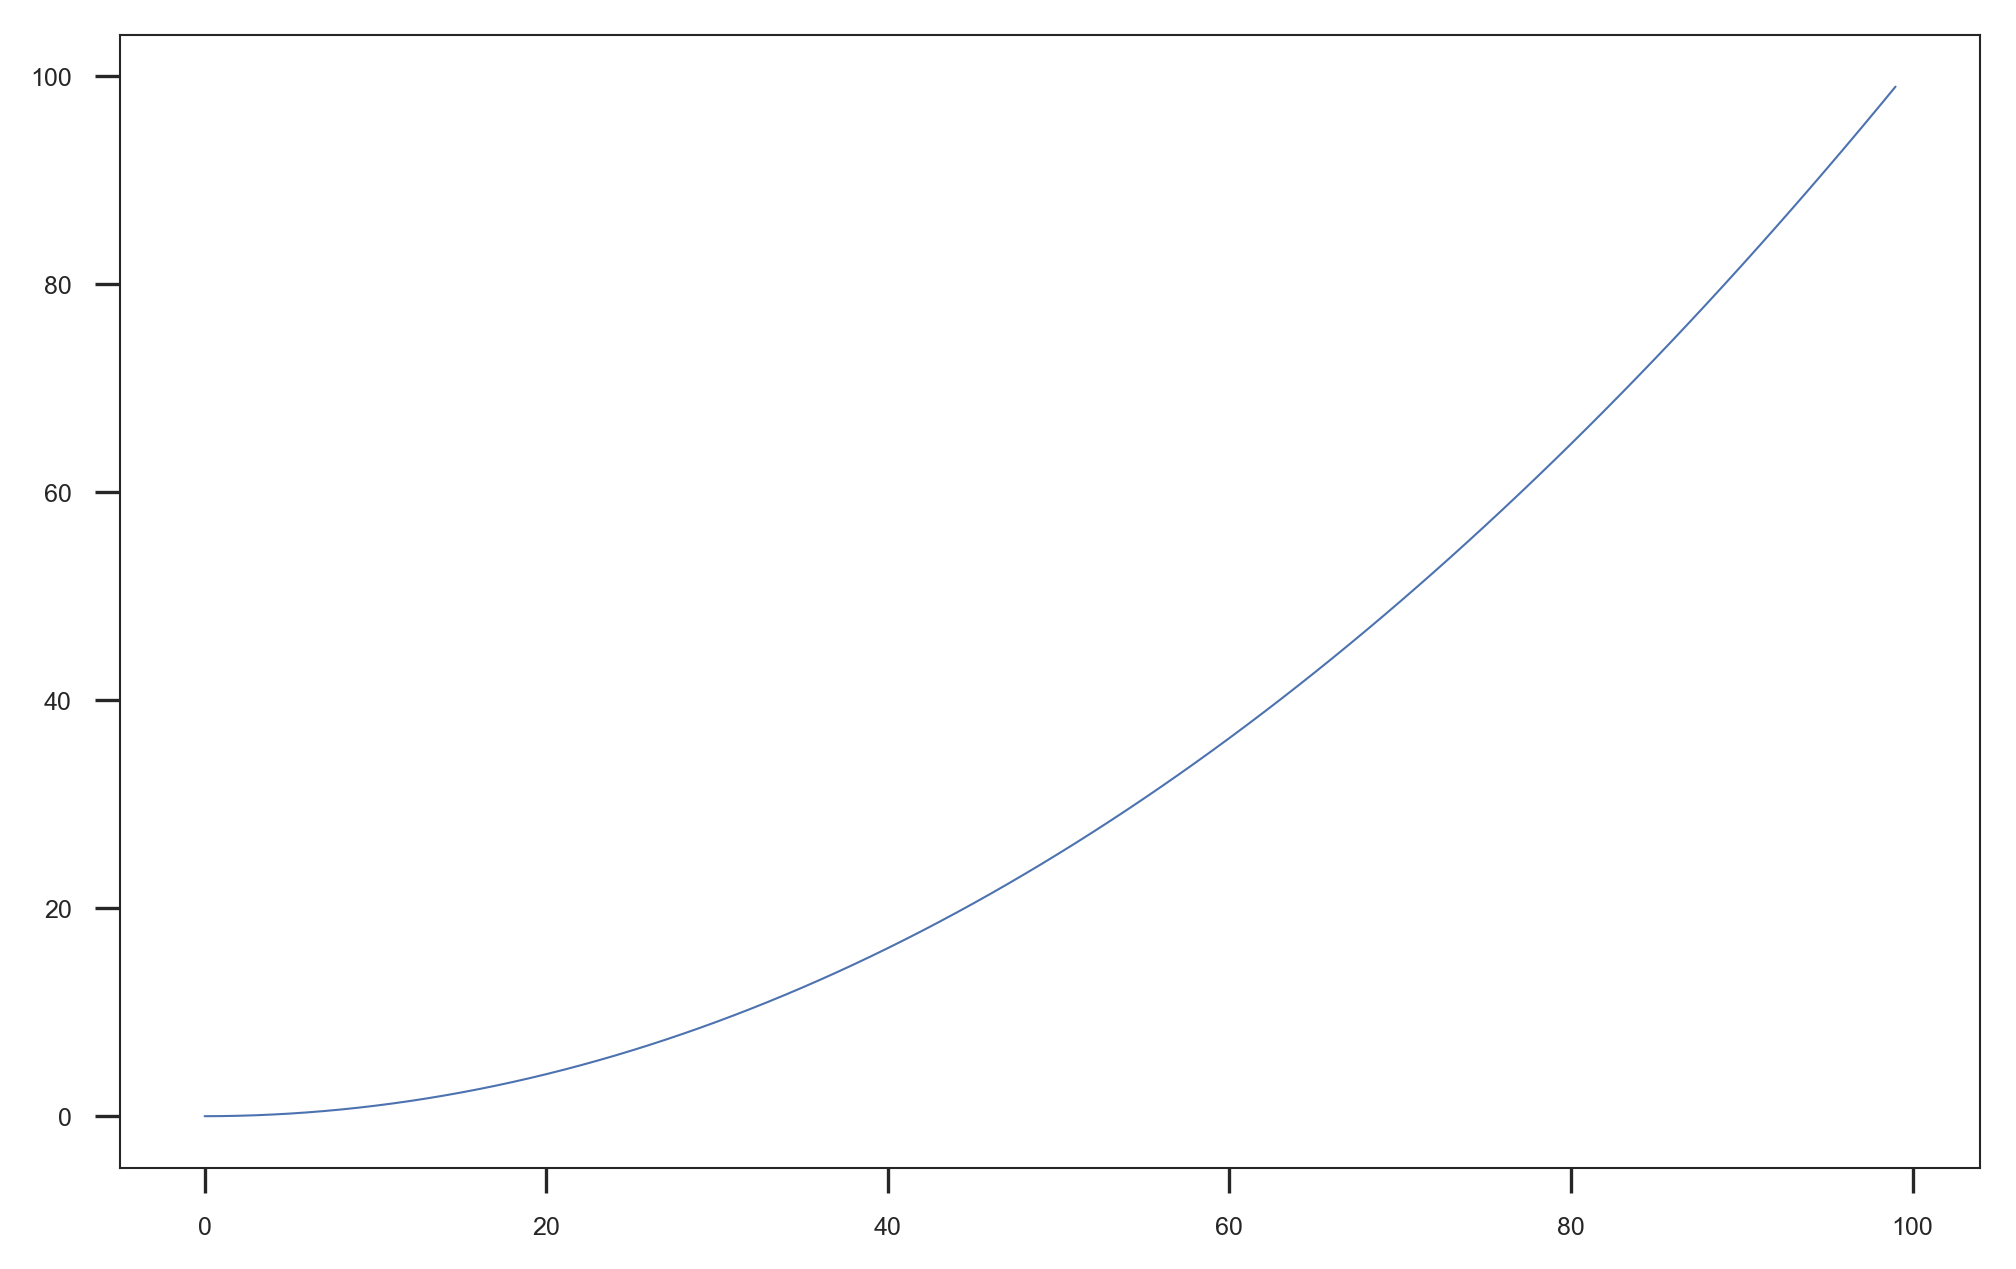
\includegraphics[width=1.1\linewidth,center]{artwork/demo.png}
  \caption{Demo figure.}
  \label{fig:demo}
\end{figure}


TODO


\section*{Discussion}

TODO


\section*{Methods}

TODO

\printbibliography

\end{document}
